
\documentclass[compress]{beamer}

%\usepackage{beamerthemesplit}
\usepackage{xmpmulti}

\usepackage{graphicx,float,wrapfig, bbm}
\usepackage{amsfonts, bbold, comment}
\usepackage{mdwlist}
\usepackage{subfigure}
\usepackage{colortbl}

\usepackage{multirow}

\pgfdeclareimage[width=\paperwidth]{mybackground}{../../common/boulder.pdf}

\newcommand{\e}[2]{\mathbb{E}_{#1}\left[ #2 \right] }
\newcommand{\ind}[1]{\mathbb{I}\left[ #1 \right] }
\newcommand{\ex}[1]{\mbox{exp}\left\{ #1\right\} }
\newcommand{\g}{\, | \,}
\newcommand{\citename}[1]{#1 }

\newcommand{\gfxs}[2]{
\begin{center}
	\includegraphics[width=#2\linewidth]{simtrans/#1}
\end{center}
}

\newcommand{\gfxq}[2]{
\begin{center}
	\includegraphics[width=#2\linewidth]{qb/#1}
\end{center}
}


\usetheme[bullet=circle,                     % Use circles instead of squares for bullets.
          titleline=true,                    % Show a line below the frame title.
          showdate=true,                     % show the date on the title page
          alternativetitlepage=true,         % Use the fancy title page.
          titlepagelogo=general_figures/culogo,              % Logo for the first page.
          % Logo for the header on first page.
          headerlogo=general_figures/boulder_cs,
          ]{UCBoulder}

\usecolortheme{ucdblack}
\title[Thinking on Your Feet]{Thinking on your Feet: Reinforcement Learning for Incremental
Language Tasks}
\author{ Jordan Boyd-Graber}
\date{Summer 2015}

\institute[Boulder] % (optional, but mostly needed)
{University of Colorado Boulder}

\AtBeginSection[] % "Beamer, do the following at the start of every section"
{ \begin{frame} \frametitle{Outline} % make a frame titled "Outline"
\tableofcontents[currentsection] % show TOC and highlight current section
\end{frame} }

\begin{document}

\frame{
\titlepage
\tiny
}


\begin{frame}{Nuremburg Trials}

\begin{columns}

\column{.5\linewidth}

    \gfxs{nuremberg_trials}{1.0}

\column{.5\linewidth}

    \begin{itemize}
        \item Dozens of defendants
        \item Judges from four nations (three languages)
\pause
        \item Status quo: speak, then translate
\pause
        \item After Nuremberg, simultaneous translations became the
          norm
\pause
        \item Long wait $\rightarrow$ bad conversation
     \end{itemize}

\end{columns}

\end{frame}



\begin{frame}{Algorithms that think on their feet}

\begin{columns}

  \column{.65\linewidth}
  \begin{itemize}
     \item Algorithms that process examples \emph{one word at a time}
       \begin{itemize}
         \item Simultaneous machine translation
         \item Trivia games
       \end{itemize}
      \item Similar structure
        \begin{itemize}
          \item Prediction
          \item Policy
        \end{itemize}
  \end{itemize}

  \column{.3\linewidth}

  \gfxs{nuremberg_translators}{.7}
  \gfxq{quizbowl}{.7}

\end{columns}

\end{frame}



\begin{frame}{Very Different Tasks, Common Foundation}

\begin{columns}
\column{.5\linewidth}
  \gfxs{pancake_robot}{.4}
  \begin{center}
  \end{center}
  
  \column{.5\linewidth}
  \begin{itemize}
    \item Reinforcement learning
    \item Machine learning / robotics framework
    \item Underused in NLP
  \end{itemize}
\end{columns}

\vspace{-.5cm}

  \begin{center}
\begin{tabular}{ccc}
\hline
  & QA & MT \\
\hline
{\bf State} & Words Seen & Foreign Words Seen \\
{\bf Reward} & Answer Accuracy & Translation Quality \\
{\bf Actions} & Answer / Wait & Translate / Wait \\
\hline
\end{tabular}

  \end{center}

\end{frame}

\section{Simultaneous Translation}

\begin{frame}{Simultaneous translation is the norm}

  \begin{columns}
    \column{.5\linewidth}
       \gfxs{nuremberg_translators}{.9}
    \column{.5\linewidth}
       \begin{itemize}
         \item Rigorous training
         \item Technological sophistication
         \item Long way from ``sentence at a time''
       \end{itemize}
  \end{columns}

\end{frame}

\begin{frame}{Why simultaneous translation really hard is}

  \begin{columns}
    \column{.5\linewidth}
      \begin{itemize}
        \item Many languages are \textsc{sov}
        \item \alert<2>{German}, Japanese, Farsi, Korean,
          \alert<3>{Yiddish}
        \item<4-> First learned system for simulatenous translation
      \end{itemize}
    \column{.5\linewidth}
      \gfxs{yoda}{.6}
  \end{columns}

  \centering

\only<4->{
\vspace{1cm}

\begin{tabular}{c@{ }c@{ }c@{ }c@{ }c@{ }c@{ }c@{ }l}
ich & bin & mit & dem & Zug & nach & Ulm & {\bf gefahren} \\
I & am & with & the & train & to & Ulm & {\bf traveled} \\
\hline
I & \multicolumn{6}{c}{\emph{(\dots\dots waiting\dots\dots)}} & {\bf traveled} by train to Ulm \\
\end{tabular}
}

\end{frame}


\begin{frame}{}

  \begin{columns}
    \column{.5\linewidth}
        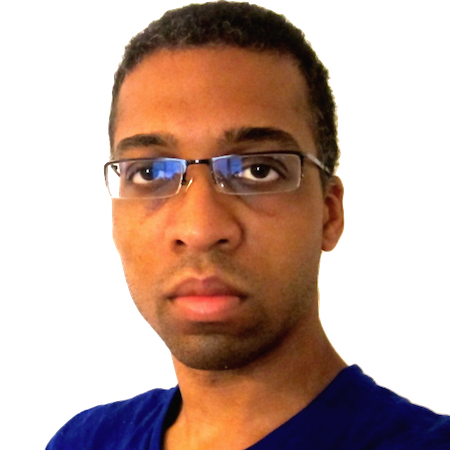
\includegraphics[width=0.9\linewidth]{general_figures/alvin}
    \column{.5\linewidth}
        \begin{block}{ {\bf \href{http://cs.colorado.edu/~jbg//docs/2014_emnlp_simtrans.pdf}{Don't Until the Final Verb Wait: Reinforcement Learning for Simultaneous Machine Translation}}}
\underline{\href{http://www.umiacs.umd.edu/~alvin/}{Alvin Grissom II}}, {\bf Jordan Boyd-Graber}, He He, John Morgan, and Hal {Daum\'{e} III}.  \emph{Empirical Methods in Natural Language Processing}, 2014
        \end{block}
  \end{columns}
\end{frame}

\begin{frame}{Solution: Predicting the Verb}

\begin{columns}

\column{.5\linewidth}
  \begin{itemize}
    \item If we can figure out the verb, we can ``complete'' the
      sentence
    \item This is provided by language models that can predict the
      next word in a sentence
    \item Instead, we'll predict the verb
  \end{itemize}

\column{.5\linewidth}

\gfxs{autocomplete}{.8}

\end{columns}

\end{frame}


\begin{frame}{Language Models of Verbs}

  \only<1>{\gfxs{verb_corpus_1}{.9}}
  \only<2>{\gfxs{verb_corpus_2}{.9}}
  \only<3>{\gfxs{verb_corpus_3}{.9}}

\end{frame}

\begin{frame}{Predicting the Verb}
\begin{itemize}
  \item Build language model for every verb
  \item Then, for any input text $x$ we can make a prediction of the verb
\begin{equation}
  \arg\max_v p(v) \prod_{i=1}^t p(x_i \g v, x_{i-n+1:i-1})
\end{equation}
\pause
  \item Most of these predictions will be totally wrong (18\%
    accuracy) \dots
  \item leading to horrible translations
\end{itemize}
\end{frame}

\begin{frame}{States and Actions}

  \begin{itemize}
    \item State
      \begin{itemize}
        \item The words we've seen
        \item Predictions
      \end{itemize}
      \pause
    \item Actions 
      \begin{itemize}
        \item Wait
        \item \alert<3>{Predict Verb and Translate}
        \item \alert<3>{Commit to Translation}
      \end{itemize}
    \end{itemize}
\end{frame}

\begin{frame}{Translations}
  \begin{itemize}
    \item Assume a ``black box''
    \item German in, English out
  \end{itemize}

\end{frame}

\begin{frame}{Consensus Translation}

  \only<1>{\begin{center}
``German in, English out'' black box
      \end{center}}

  \only<2>{\gfxs{consensus_0}{.8}}
  \only<3>{\gfxs{consensus_1}{.8}}
  \only<4>{\gfxs{consensus_2}{.8}}
  \only<5>{\gfxs{consensus_3}{.8}}
  \only<6>{\gfxs{consensus_4}{.8}}

\end{frame}

\begin{frame}{Scoring one Translation}
  \begin{center}
    Bilingual Evaluation Understudy (BLEU)
\end{center}
  \only<1>{\gfxs{bleu_ex}{.8}}
  \only<2>{\gfxs{bleu_correlation}{.6}}
\end{frame}


\begin{frame}{Scoring a series of Translations}
  \begin{center}
    Bilingual Evaluation Understudy (BLEU)
\end{center}
  \only<1>{\gfxs{integral_0}{.95}}
  \only<2>{\gfxs{integral_1}{.95}}
\end{frame}



\begin{frame}{Comparing Policies}

  \only<1-7>{\vspace{4.75cm}}
  \only<8-14>{\vspace{3.3cm}}
  \only<15-21>{\vspace{2cm}}

  \only<1,8,15,22>{\gfxs{reward_example_0}{.8}}
  \only<2,9,16,23>{\gfxs{reward_example_1}{.8}}
  \only<3,10,17,24>{\gfxs{reward_example_2}{.8}}
  \only<4,11,18,25>{\gfxs{reward_example_3}{.8}}
  \only<5,12,19,26>{\gfxs{reward_example_4}{.8}}
  \only<6,13,20,27>{\gfxs{reward_example_5}{.8}}
  \only<7,14,21,28>{\gfxs{reward_example_6}{.8}}
\end{frame}




\begin{frame}{Imitation Learning}

  \begin{columns}
    \column{.5\linewidth}
       \gfxs{imitation_fold}{.8}
       \gfxs{imitation_drive}{.8}
    \column{.5\linewidth}
    \begin{itemize}
      \item Given all the predictions that we make (and the resulting
        translations) \dots
      \item Discover the optimal in hindsight policies
      \item Goal: Teach our algorithm to think on its feet
      \item Challenge: Represent states in a way that will generalize
        \pause
      \item \textsc{searn}: \underline{Se}arching to L\underline{earn}
    (Daum\'e \& Marcu, 2006)
    \end{itemize}

  \end{columns}

\end{frame}

\begin{frame}{Experimental Setup}

  \begin{itemize}
    \item \textsc{denews} corpus
      \begin{itemize}
        \item News snippets
        \item Some formulaic
        \item Some surprising
      \end{itemize}
    \item Only verb-final sentences
    \item Some compromises with translation system (to make sure verbs appeared)
  \end{itemize}

\end{frame}



\begin{frame}{Comparing Policies}

  \gfxs{cummulative}{.6}

\end{frame}

\begin{frame}{Learned Policy with Accumulated Reward}

  \only<1>{\gfxs{compare_line_batch}{.8}}
  \only<2>{\gfxs{compare_line_batch_monotone}{.8}}
  \only<3>{\gfxs{compare_line_batch_monotone_opt}{.8}}
  \only<4>{\gfxs{compare_line_all}{.8}}
\end{frame}


\begin{frame}{Example Sentence}

  \gfxs{ex_imperfect}{.7}

\end{frame}

\begin{frame}{Future Steps}

  \begin{itemize}
    \item Richer translation model
    \item Paraphrase database
    \item Better reward (e.g., MEANT)
    \item Verb prediction through argument structure
  \end{itemize}

\end{frame}

\section{Quiz Bowl}

\begin{frame}{Other Tasks with Similar Structure}
	\begin{columns}

	\column{.5\linewidth}
	\begin{itemize}
		\item Game called ``quiz bowl''
		\item Two teams play each other
		\begin{itemize}
			\item Moderator reads a question
			\item When a team knows the answer, they signal (``buzz'' in)
			\item If right, they get points; otherwise, rest of the question is read to the other team
		\end{itemize}
		\item Hundreds of teams in the US alone
	\end{itemize}

	\column{.5\linewidth}
	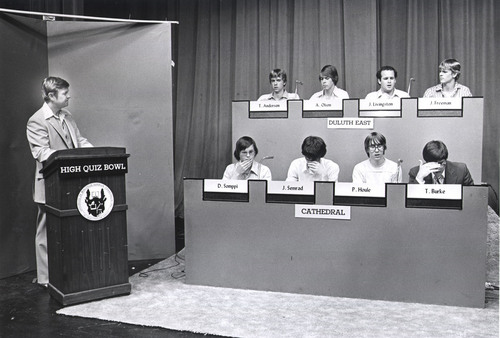
\includegraphics{qb/quizbowl}

	\end{columns}

\end{frame}



\begin{frame}
	\frametitle{Humans doing Incremental Classification}

	\begin{columns}
		\column{.5\linewidth}

		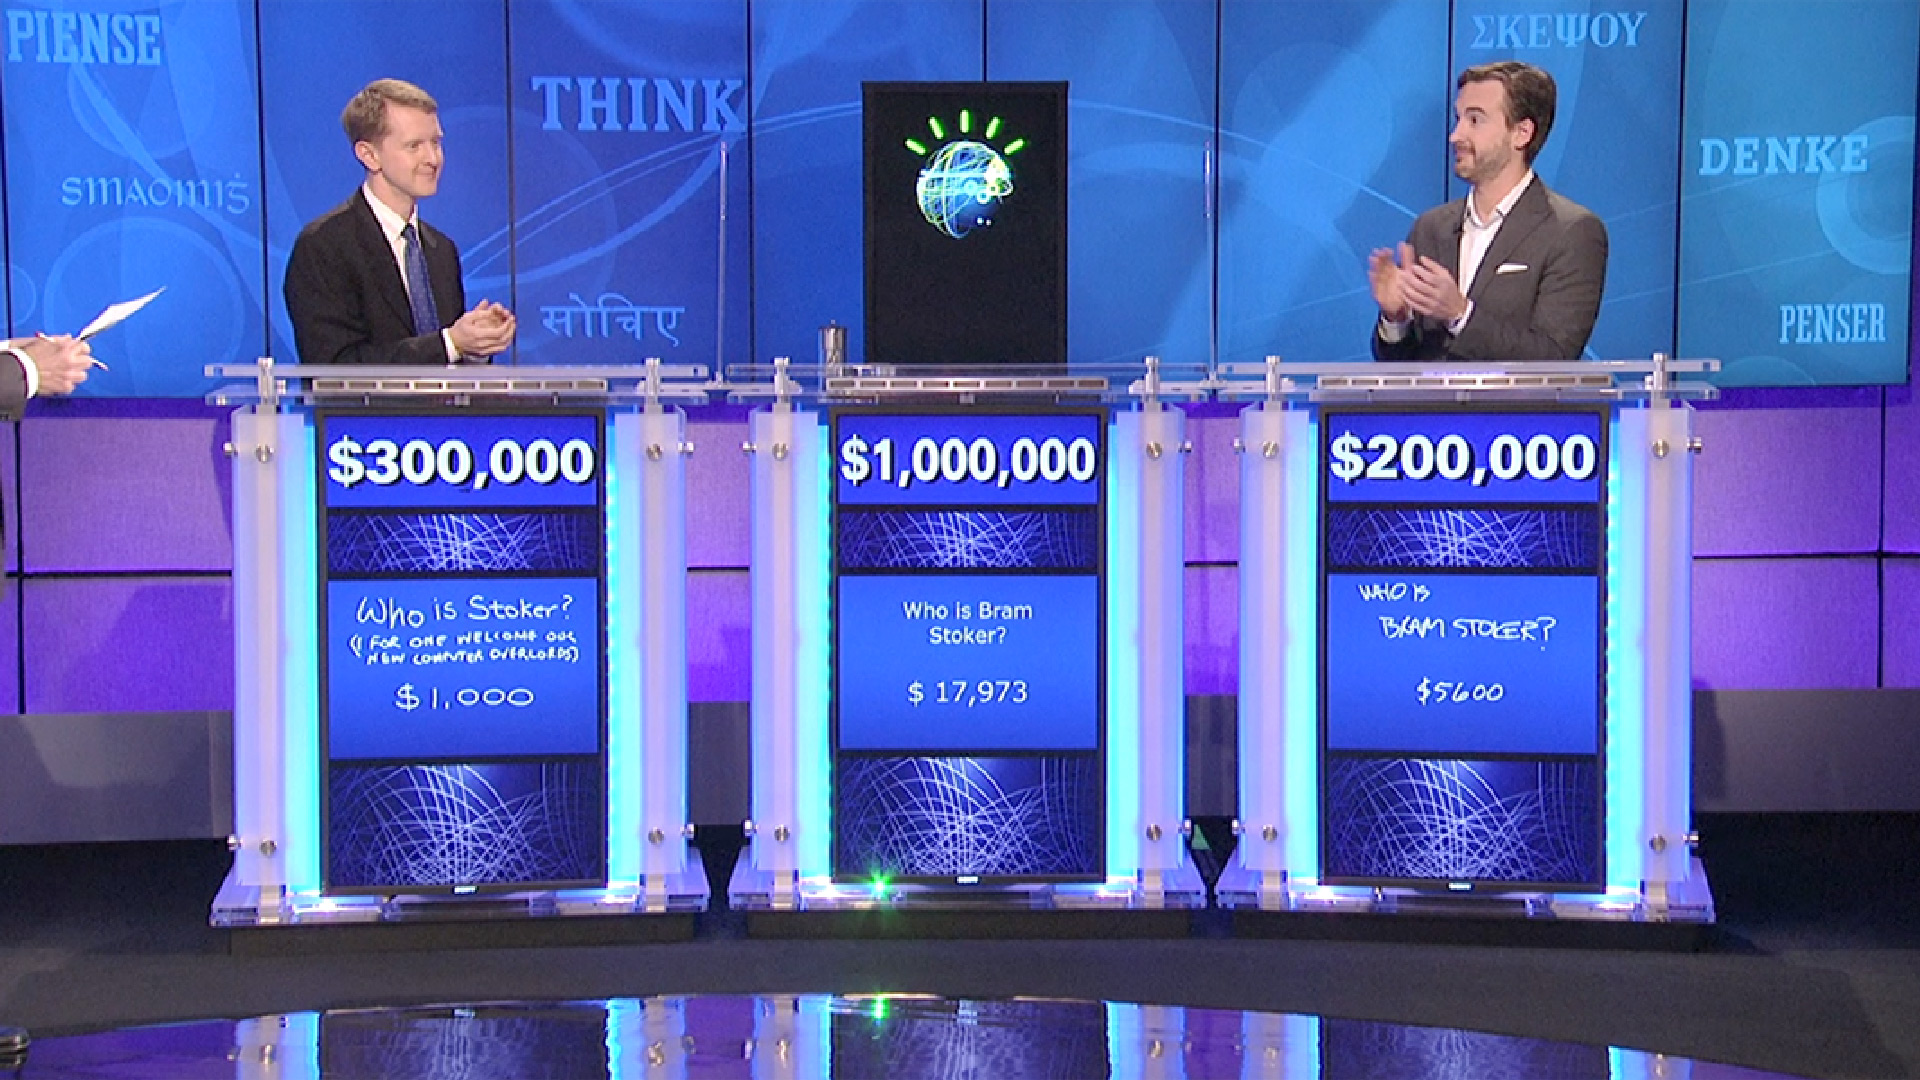
\includegraphics[width=1.0\linewidth]{qb/jeopardy}


		\column{.5\linewidth}
		\begin{itemize}
			\item This is {\bf not} Jeopardy \cite{ferruci-10}
			\item There are buzzers, but players only buzz
                          at the question end
			\item Doesn't discriminate knowledge
			\item Quiz bowl is pyramidal
                        \item Watson must decide to answer {\bf once}, after
                          complete question
                        \item Quiz Bowl: decide after each word
		\end{itemize}

	\end{columns}

\end{frame}




\section{Conclusions}

\begin{frame}{What I'd Like to Know}

  \begin{itemize}
    \item How to better predict verbs (and other things)
    \item Better speed / accuracy metrics
    \item Correcting errors
    \item Dealing better with relative clauses
  \end{itemize}

\end{frame}



\frame{

	\frametitle{Thanks}

}



\begin{frame}{References}
\bibliographystyle{style/acl}
\tiny
\bibliography{bib/journal-full,bib/jbg}
\end{frame}




	

\begin{frame}
	\frametitle{Learning which Features are Useful}

	\begin{itemize}
		\item Use how humans these data as a prior for supervised maxent model~\cite{daume-04}
		\item Prior for label $a$ and feature $f$ is a function of the number of buzzes $b$ and tf-idf~\cite{salton-68}
\begin{equation}
  \left[ \vphantom{\frac{a}{b}}\alpha \alert<4>{\ind{ b(a,f) > 0}} + \beta \alert<3>{ b(a,f)} + \gamma
  \right] \alert<2>{\mbox{tf-idf}(a,f)} .
\label{eq:meanweight}
\end{equation}
		\begin{itemize}
			\item $\alpha$, $\beta$, and $\gamma = 0$: na\"ive zero prior
			\item $\alpha$ and $\beta = 0$: linear transformation of the mean
			\item $\alpha$ and $\gamma = 0$: number of buzzes times tf-idf value of the features
		\end{itemize}

	\end{itemize}

\end{frame}

\begin{frame}
	\frametitle{Using buzzes as a prior}

\begin{equation*}
  \left[ \vphantom{\frac{a}{b}}\alpha \ind{ b(a,f) > 0} + \beta b(a,f) + \gamma
  \right] \mbox{tf-idf}(a,f) .
\end{equation*}

\begin{center}
\begin{tabular}{cccccc}
Answers & Weighting & $\alpha$ & $\beta$ & $\gamma$ & Error\footnote{Buzz and tf-idf computed on training data; grid search on dev data; error on test data} \\
\hline
\multirow{5}{*}{100} & zero & - & - & - & 0.22 \\
& tf-idf & - & - & 8.3 & 0.08 \\
&  buzz-binary & 10.7 & - & - & {\bf 0.06} \\
&  buzz-linear & - &  1.1 & - & 0.10 \\
& buzz-tier & - & 1.6 & 0.5 & 0.07 \\
\hline
\end{tabular}
\end{center}
\end{frame}





\begin{frame}
	\begin{center}

\vspace{-.6cm}
\begin{figure}[tb]
\centering

\subfigure[Buzzes over all Questions]{
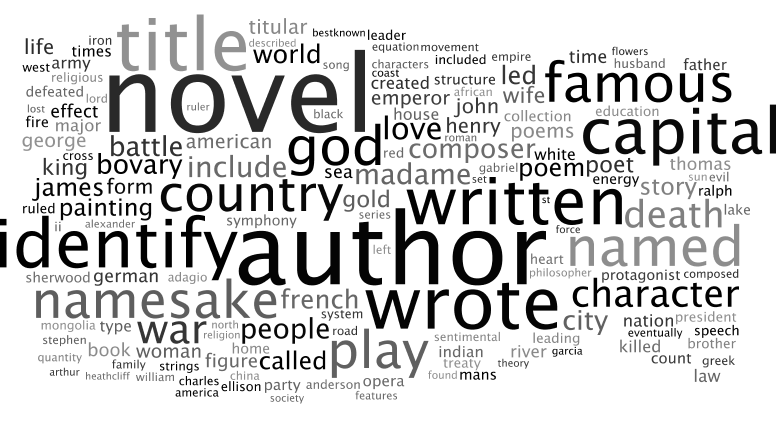
\includegraphics[width=0.6\linewidth]{qb/buzz_cloud}
\label{fig:buzz_cloud}
}

\subfigure[Wuthering Heights Question Text]{
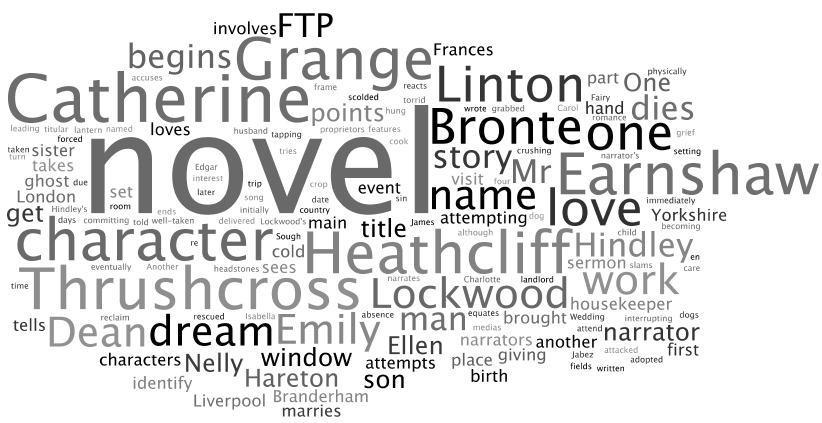
\includegraphics[width=0.45\linewidth]{qb/wuthering_heights_question}
\label{fig:wh_question}
}
\subfigure[Buzzes on Wuthering Heights]{
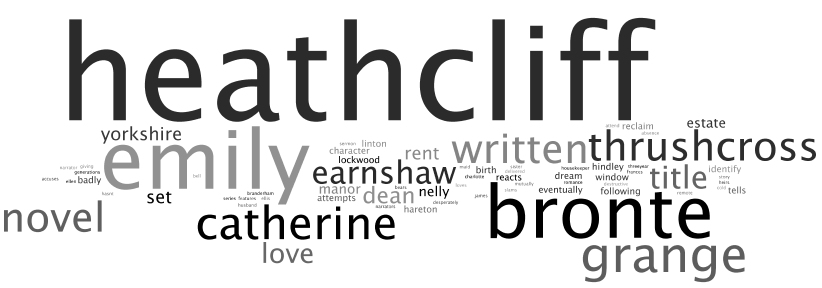
\includegraphics[width=0.45\linewidth]{qb/wuthering_heights_buzz}
\label{fig:wh_buzz}
}
\end{figure}


	\end{center}

\end{frame}



\begin{frame}
	\frametitle{Accuracy vs. Speed}

	\begin{center}
	  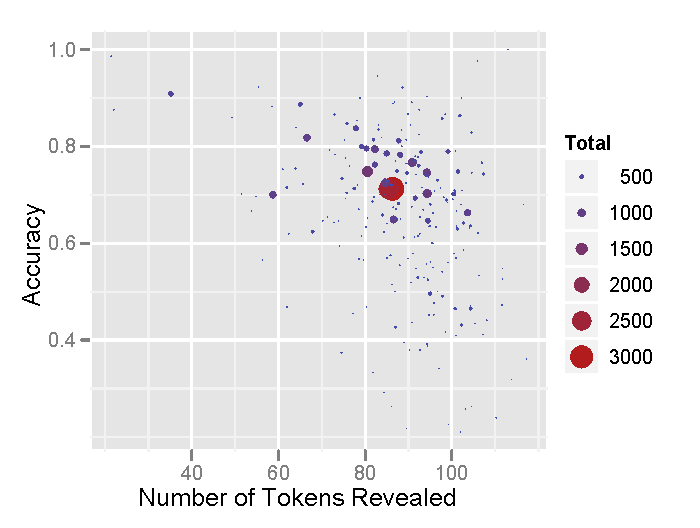
\includegraphics[width=0.8\linewidth]{qb/accuracy_vs_speed}
	  \end{center}

\end{frame}

\begin{frame}{How we could translate a sentence}

\only<1>{\gfxs{example_3}{.9}}
\only<2>{\gfxs{example_4}{.9}}
\only<3>{\gfxs{example_5}{.9}}
\only<4>{\gfxs{example_6}{.9}}
\only<5>{\gfxs{example_7}{.9}}
\only<6>{\gfxs{example_8}{.9}}
\only<7>{\gfxs{example_9}{.9}}
\only<8>{\gfxs{example_10}{.9}}
\only<9>{\gfxs{example_11}{.9}}
\only<10>{\gfxs{example_12}{.9}}
\only<11>{\gfxs{example_13}{.9}}
\only<12>{\gfxs{example_14}{.9}}
\only<13>{\gfxs{example_15}{.9}}
\only<14>{\gfxs{example_16}{.9}}
\only<15>{\gfxs{example_17}{.9}}
\only<16>{\gfxs{example_18}{.9}}
\only<17>{\gfxs{example_19}{.9}}
\end{frame}




\end{document}
